\documentclass[english]{upeeei}
\usepackage[latin9]{inputenc}
\setcounter{secnumdepth}{3}
\setcounter{tocdepth}{3}
\usepackage[active]{srcltx}
\usepackage{units}
\usepackage{parskip}
\usepackage{graphicx}
\usepackage{subfigure} 
\usepackage{url}  
%\usepackage{stfloats}  
\usepackage{amsmath}   
\usepackage{array}
\usepackage{caption}
\usepackage{afterpage}
\usepackage{textcomp}
\usepackage{lscape}
\usepackage{stfloats}
\usepackage{hyphenat}
\usepackage{makeidx}
\usepackage{amssymb}
%\usepackage{underscore}
\fnbelowfloat
\usepackage{times}
\usepackage{multirow}
%\usepackage{float}
\usepackage{circuitikz}
\usepackage[backend=bibtex,bibstyle=ieee,citestyle=numeric-comp]{biblatex}
\addbibresource{Proposal_Part1.bib}
\usepackage{pgfplots}
%\usepackage{arydshln}
\pgfplotsset{width=7cm,compat=1.5.1}
\renewcommand*{\bibfont}{\small}

\newcolumntype{L}[1]{>{\raggedright\let\newline\\\arraybackslash\hspace{0pt}}m{#1}}
\newcolumntype{C}[1]{>{\centering\let\newline\\\arraybackslash\hspace{0pt}}m{#1}}
\newcolumntype{R}[1]{>{\raggedleft\let\newline\\\arraybackslash\hspace{0pt}}m{#1}}

\newcommand\ddfrac[2]{\frac{\displaystyle #1}{\displaystyle #2}}
\pgfplotsset{compat=1.14}

\makeatletter

%%%%%%%%%%%%%%%%%%%%%%%%%%%%%% LyX specific LaTeX commands.
\providecommand{\LyX}{L\kern-.1667em\lower.25em\hbox{Y}\kern-.125emX\@}
%% Because html converters don't know tabularnewline
\providecommand{\tabularnewline}{\\}

\@ifundefined{showcaptionsetup}{}{%
 \PassOptionsToPackage{caption=false}{subfig}}
\usepackage{subfig}
\makeatother

\usepackage{babel}

\begin{document}
%%% UP EEEI undergraduate project template
%% v0.1 by Louis P. Alarcon 11/22/2011
%%
%% LyX template - use with the following files:
%% 	uct10_new.clo, uct11_new.clo, uct12_new.clo, upeeei.cls, upeeei.layout
%%
%% Place project title here
\title{Design of a Raspberry Pi Based Flight Controller for Multirotor Unmanned Aerial Vehicles} 

%%
%% Author information

\author{
%% Use \vspace to separate each member
%% Put your names here in alphabetical order
\\Louie Isaniel Cachola Henson \\ 2014-30227 \\ \emph{B.S. Computer Engineering}
}

%%
%% Month and year of submission/graduation
\degreeyear{2021} 
\degreesemester{January} 

% Put your advisers here:
\chair{Professor Charleston Dale Ambatali
\\
Roxanne P. De Leon, ECE, MTM
} 
%\othermembers{John Richard Ereso Hizon\\ 
%Joel Joseph Sarco Marciano, Jr.} 
\numberofmembers{1} 

\field{Electrical/Computer/Electronics and Communications Engineering} 
\campus{Diliman} 

\maketitle
% \approvalpage 
% \copyrightpage 
\begin{abstract} 

%Your abstract goes here...


Multirotor unmanned aerial vehicles (or drones) are quick and versatile, often 
proving to be a great asset for various purposes. It is because of this that drones have been integrated into
more industries and fields of study. This necessitates the development of flight controllers that are
cost-effective, versatile and easy to develop. Meanwhile, the Raspberry Pi has shown steady development, quickly
growing more powerful and versatile with each model released. It allows for rapid prototyping while remaining
small and relatively inexpensive, making it a good fit to be a flight controller. Despite this, there are no
publicly available open source flight controllers that are based solely on the Raspberry Pi.
The goal of this project is to develop a flight controller that is readily compatible with the Raspberry Pi, 
thereby taking advantage of the Raspberry Pi's versatility and low cost. This is in line with the Advanced 
Defense and Aerospace Materials (ADAM) R\&D's Project Diosa, where the goal is to develop a multirotor UAV using 
low cost materials. 


\end{abstract}

\begin{frontmatter}
\setlength{\parskip}{0pt}
\tableofcontents
%\listoftables
\listoffigures
\end{frontmatter}
\def\MASTERDOC{true}

\chapter{Introduction}
Unmanned aerial vehicles (UAVs) continue to be integrated into increasingly diverse environments and
fields. From photography and cinematography, all the way to military applications and even disaster risk reduction and 
management. They are especially useful for reducing the amount of risk that personnel experience by flying to places that 
pose a significant hazard to personnel \cite{ICNSC2010}. Advanced Defense and Aerospace Materials (ADAM) R\&D's Project
Diosa aims to develop a functional but low cost multirotor unmanned aerial vehicle (UAV) for use in humanitarian aid
\cite{diosa2020}. As a part of that endeavor, this project aims to develop a cost effective but versatile flight 
controller capable of being integrated into Project Diosa.
\begin{figure}[h]
    \centering
    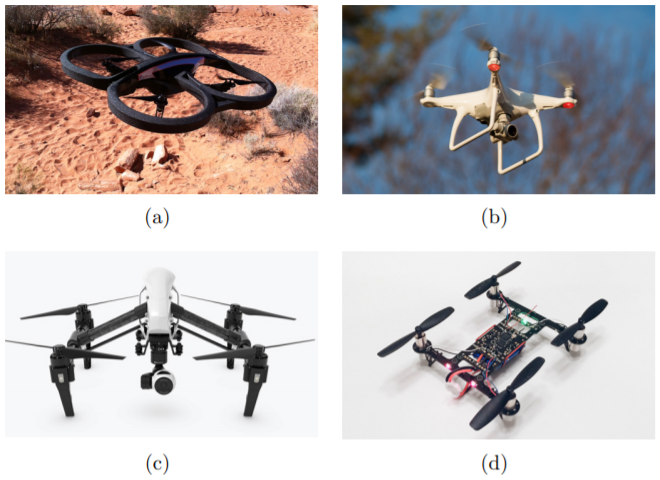
\includegraphics[scale=0.5]{images/droneExamples.PNG}
    \caption{Examples of multirotor UAVs \cite{zimmerman2016}}
    \label{fig:droneExamples}
\end{figure}

\section{An Overview of UAVs}
\begin{figure}[h]
    \centering
    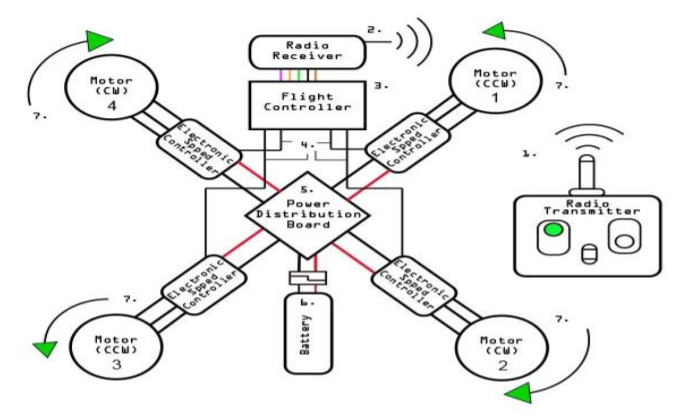
\includegraphics[scale=0.7]{images/fc_diag.PNG}
    \caption{Diagram of a quadcopter with radio transmitter\cite{fcDesign2019}}
    \label{fig:baseQuad}
\end{figure}
One might view the UAV as a black box where we input certain instructions and the UAV provides output in the form of
movement. Looking further into the system, we can see quite a bit of complexity with the internal subsystems that need
to interact in order for the UAV to achieve stable flight.
One of the most common types of multirotor UAVs is the quadcopter or quadrotor, so named because it uses four motors to
move around. The system diagram of a quadcopter may be seen in figure \ref{fig:baseQuad}. Some of the vital parts that all
multirotors have in common are:
\begin{enumerate}
    \item Motors
    \item Electronic speed controllers (ESCs)
    \item Battery
    \item Radio transceiver
    \item Flight controller
\end{enumerate}
The \textbf{motors} are the primary and often sole method of movement for the UAV. Coupled with propellers, they rotate at
very high velocities in order to generate lift. These motors are often brushless and generate high torque in exchange for
taking up a large amount of current \cite{fcDesign2019}. 
\newline
\newline
The \textbf{electronic speed controllers} are connected directly to the motors and allow you to control them through PWM
signals from the flight controller. There is typically one ESC for each motor \cite{zimmerman2016}. The ESC we will be 
using for the project is a 4-in-1 ESC board that can control four motors from one board. This was chosen as it was less
costly and more lightweight than using individual ESC modules. It is important to note that although the flight controller
can send data to the ESCs, the ESCs cannot provide direct feedback.
\newline
\newline
UAVs typically use lithium polymer \textbf{batteries}. Lithium polymer batteries are one of the densest commercially
available batteries in terms of energy \cite{LiPoly}. Because of this, they are lightweight and can provide the large 
amounts of current that is needed by the motors. In addition, the batteries also power the flight controller as well as
other onboard peripherals. In some instances, the flight controller may even read the voltage of the battery with respect to
its maximum operating voltage, thereby getting a sense of the remaining battery capacity.
\newline
\newline
The \textbf{radio transceiver} is the piece of hardware that allows the UAV to communicate with a base station. This allows
a pilot to send commands to the UAV and receive data such as telemetry or GPS coordinates \cite{zimmerman2016}.
\newline
\newline
The \textbf{flight controller} is, as its name suggests, the central device that controls how the UAV moves and reacts to certain
stimuli. The flight controller contains multiple sensors including (but not limited to) a gyroscope, accelerometer, and
barometer. These sensors allow the flight controller to get a sense of its orientation in 3D space \cite{zimmerman2016}. The
flight controller sends instructions to the ESCs in order to vary the throttle of each motor.

\section{A Deeper Look Into Flight Controllers}
Because of the growing interest in UAVs, various flight
controllers have been developed such as the microcontroller-based Multiwii \cite{MultiwiiFC} and PixHawk \cite{RPiMavlink2019}.
Microcontroller based flight controllers are ideal because they are lightweight, low-cost, and are generally versatile enough
to accomodate the peripherals that a flight controller needs in order to function properly. On top of this, these flight controllers
are often open-source and relatively simple to prototype with. However, due to the limited processing power available to 
microcontroller based flight controllers, higher level functions such as automated navigation or mapping are often impossible 
without the help of an onboard computer (often a Raspberry Pi) communicating directly with the flight controller 
\cite{RPiMavlink2019,Redtail2017,Dowling2018,Navio2,AirPy}.
\begin{figure}[h]
    \centering
    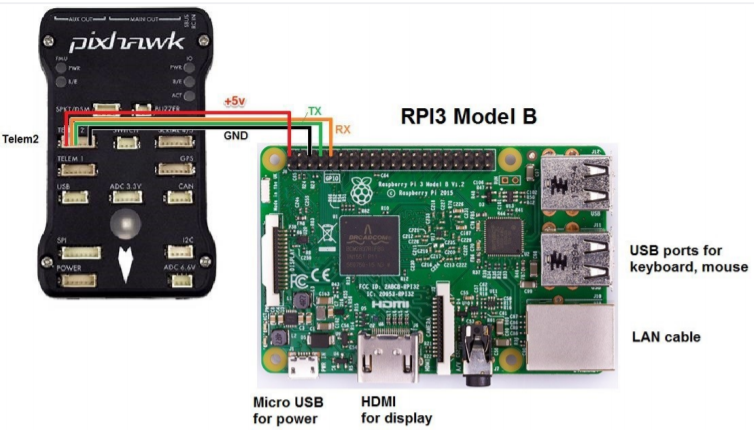
\includegraphics[scale=0.5]{images/phawkToPi.PNG}
    \caption{Connecting a Pixhawk flight controller to a Raspberry Pi \cite{RPiMavlink2019}}
    \label{fig:phawkToPi}
\end{figure}
Curiously, while there are numerous flight controllers based off of microcontrollers, there are no publicly available flight 
controllers that directly utilize an onboard computer to interface with the electronic speed controllers, thereby skipping
the microcontroller entirely. Doing so would not only lower the cost of producing the flight controller, but it would also
reduce the flight controller's size and weight while still allowing access to higher level UAV functions. A solution to this
would be to develop a flight controller board built around the Raspberry Pi 4, which is the latest and currently most powerful
version of the Raspberry Pi line of computers. Doing so would involve designing and fabricating the flight controller board (with
the necessary peripherals) as well as modeling and programming the control system. In order to make the UAV easy to mass produce 
and more affordable, production cost will be prioritized while designing the flight controller. 


\chapter{Review of Related Work}
As mentioned previously, a vast majority of commercially available flight controllers are based on microcontrollers. In order to
adapt this technology to single board computers such as the Raspberry Pi, it would serve well to examine microcontroller based
implementations. We will first look into the system architecture and design on a hardware level before moving on to how to model
the control system and program it into the hardware.
\section{Hardware Design}
Looking into open-source microcontroller-based flight controllers, two of the most prominent ones are the MultiWii \cite{MultiwiiFC}
and the PixHawk family of flight controllers \cite{RPiMavlink2019}. The MultiWii is the more dated of the two systems and the PixHawk
may also trace its origins to it. The MultiWii was
developed to use the Arduino line of microcontrollers as a base though it can also run on other select microcontrollers. It also
supports a variety of inertial measurement units (IMUs), which are sensor modules that carry an accelerometer and gyroscope and,
for some modules, even a magnetometer or barometer \cite{zimmerman2016}. Figure \ref{fig:multiwiiCktDiagram} illustrates the circuit
diagram of a basic MultiWii quadrotor UAV. In this digram, we can see that the flight controller is connected to four electronic speed
controllers (ESCs) which then control the motors directly. The flight controller takes inputs from a receiver, detailing the levels
of throttle, roll, pitch, and yaw as well as a few auxiliary channels which may be used for other functions such as LEDs or arming
the motors. The flight controller also makes use of an IMU in order to get a sense of its orientation. Along with the signals from
the receiver, it feeds this data into a PID loop (which will be discussed further on in this document) in order to maintain stable flight
\cite{zimmerman2016}. Thus, we can infer the most important parts of a flight controller; the flight controller board and the IMU.
\begin{figure}[h]
    \centering
    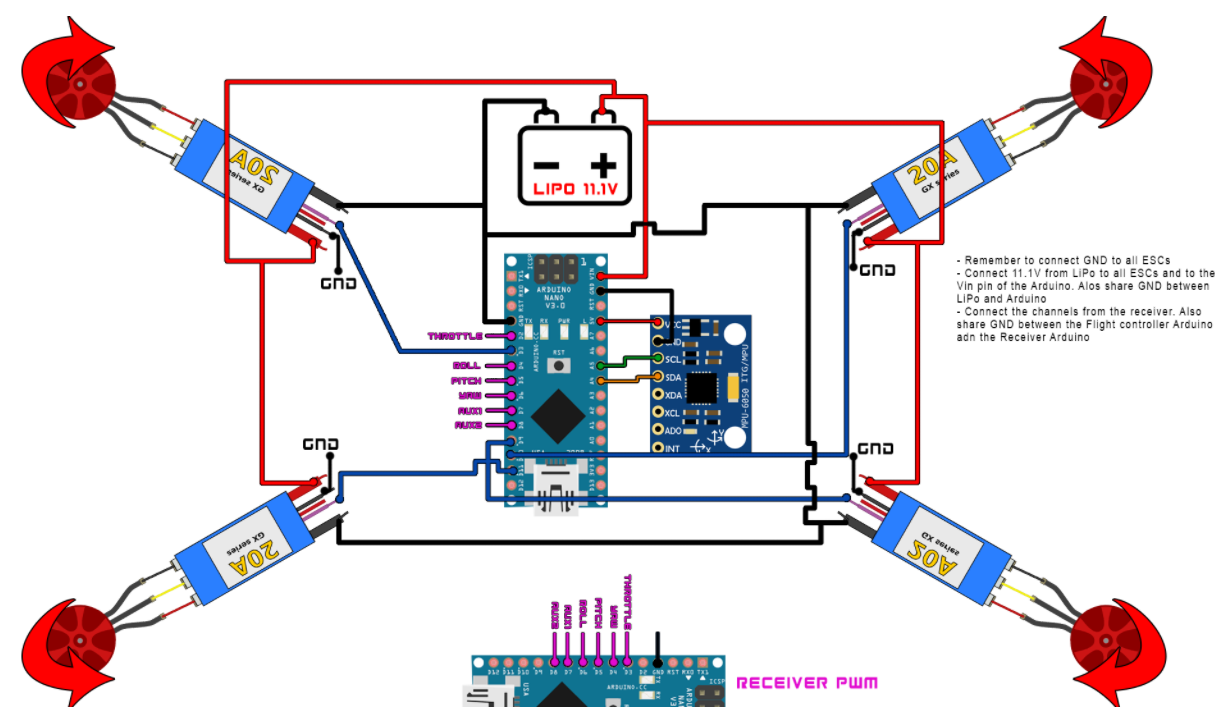
\includegraphics[scale=0.5]{images/multiwii diagram.PNG}
    \caption{Circuit diagram of basic MultiWii multirotor UAV \cite{MultiwiiFC}}
    \label{fig:multiwiiCktDiagram}
\end{figure}
\newline
\newline
Taking a step further, Sigalos et al. verify our inference in their paper entitled "Design of a Flight Controller and Peripherals 
for a Quadcopter" \cite{fcDesign2019}. As seen in figure \ref{fig:baseQuad}, the diagram is very similar to that of the base MultiWii. 
The biggest difference would be the addition of a power distribution board. The power distribution board is essentially just a circuit board
where the ESCs may be connected together. This would allow us to use less wires, thereby making the physical system tidier and thus 
easier to manage. It is also important to note that the battery voltage must be stepped up or down depending on the working voltage of
the chosen controller. In the case of the MultiWii, the battery used is a 11.1V Lithium Polymer battery. The author states that a voltage
converter was no longer needed as 11.1V is within the acceptable input voltage range of the Arduino Nano which the implemented MultiWii
uses. The Arduino Nano also already comes with an internal voltage regulator capable of stepping down the 11.1V to a more manageable
voltage. This, however, is not the case when working with the Raspberry Pi, where the input voltage must not exceed 5.1V. Thus, a
voltage regulator must be integrated into the flight controller.

Zimmerman illustrates this more clearly in their thesis "Flight Control and Hardware Design of Multi-Rotor Systems". In figure 
\ref{fig:detailed_quad_block_diagram}, the microcontroller used in the flight controller has a working voltage of 3.3V, which is a far cry
from the 11.1V input voltage. In order to compensate for this, they use a low dropout regulator to step the input voltage down to 3.3V. It
is also important to note that the microcontroller communicates both with the IMU and radio receiver via SPI. The designed flight controller
also has interfaces for PPM and UART which, as seen from the electrical architecture, were used for sonar and lidar respectively. Lidar and
sonar, however, are not vital to the UAV's operation and are treated as peripherals. It is also to be noted that this implementation does
not have an available I2C interface, something that the Raspberry Pi supports natively. The presence of an I2C interface would allow the
UAV to access more sensors or external modules should they become necessary for the UAV's application.
\begin{figure}[h]
    \centering
    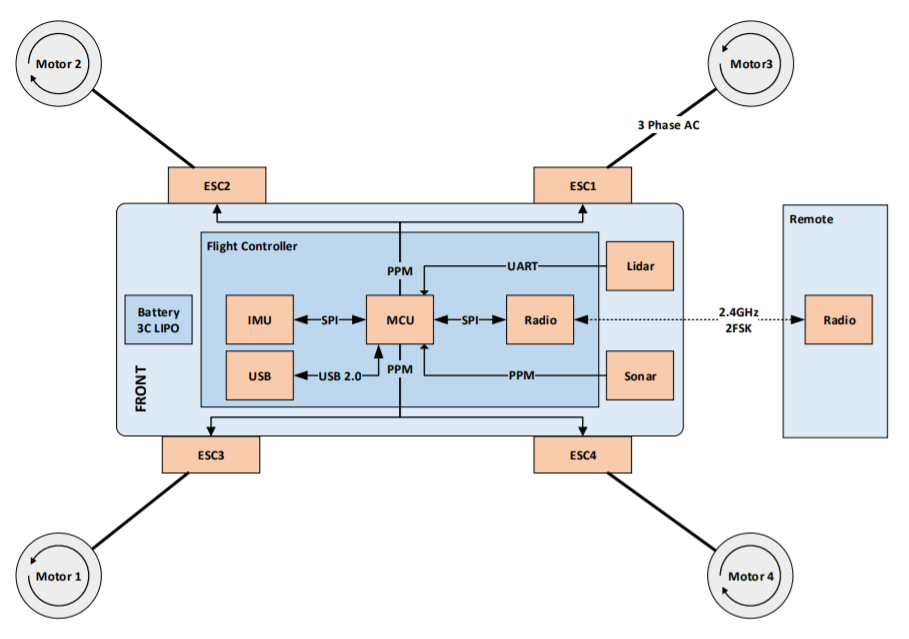
\includegraphics[scale=0.45]{images/zimmerman_high_level.PNG}
    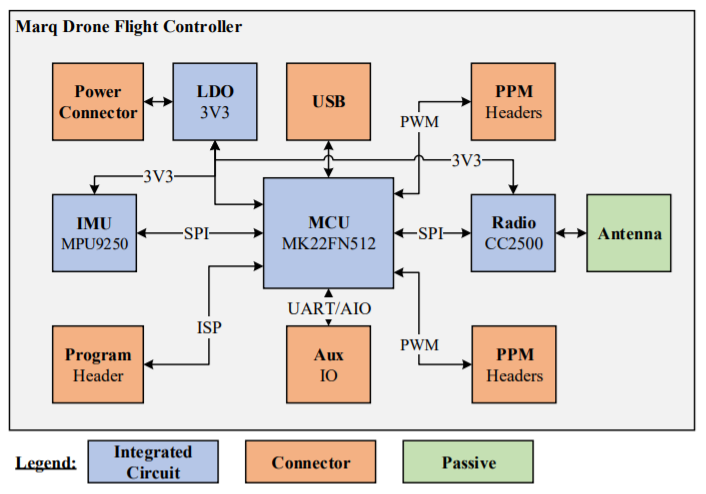
\includegraphics[scale=0.45]{images/fc_block_diagram_detailed.PNG}
    \caption{Electrical architecture diagram (left) and corresponding flight controller block diagram (right)\cite{zimmerman2016}}
    \label{fig:detailed_quad_block_diagram}
\end{figure}
\newline
\newline
Perhaps the device that best resembles what this project is trying to accomplish is the Navio2 \cite{Navio2}. Developed by a company called
Emlid, the Navio2 was designed to plug directly onto the Raspberry Pi, allowing it to function as a flight controller in and of itself. It
has two built-in IMUs as well as a barometer and a GPS module. It also supports UART as well as I2C. It does not have a built in power
module and thus any input voltage larger than 5.1V must still be stepped down accordingly. Because the Navio2 was developed for an older
version of the Raspberry Pi (namely the Raspberry Pi 2), it still needs to account for the lack of processing power. It does this by
making use of an integrated microcontroller to handle the low-level functions such as processing the PPM input from the radio receiver.
Ultimately, the Navio2 was designed more to be a solution for easy-to-use autopilot rather than a standalone flight controller. 
\begin{figure}[h]
    \centering
    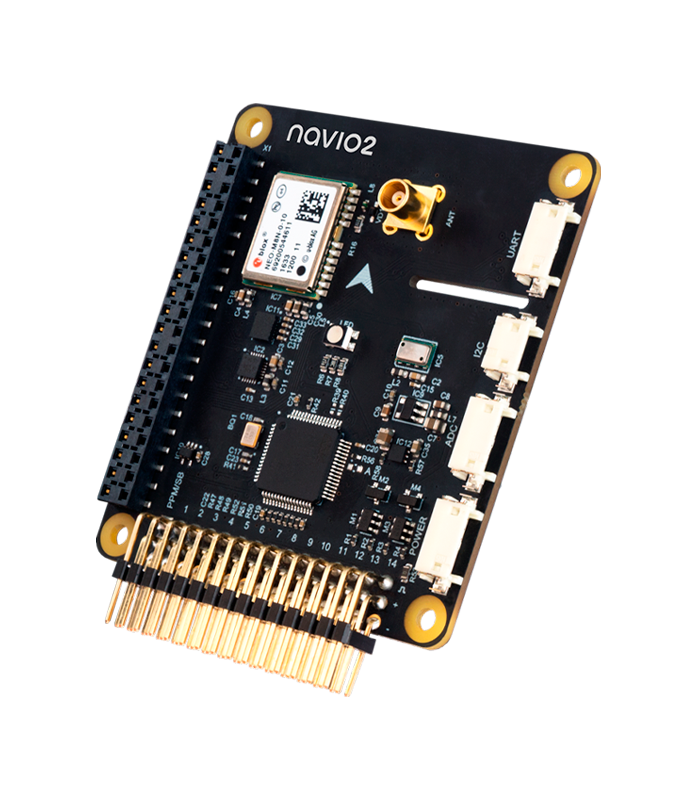
\includegraphics[scale=0.3]{images/Navio2Elements_main.png}
    \caption{Navio2 Raspberry Pi hat \cite{Navio2}}
    \label{fig:navio2}
\end{figure}

\section{Control System Design and Programming}
In typical multirotor UAV designs, the motor positions are static with respect to each other. This means that it is not possible to change
the direction of an individual motor in order to influence flight. Instead, the UAV changes the angular velocity, $\omega$, of each motor according to
the direction the pilot would like to go \cite{fcDesign2019}. Figure \ref{fig:motor_signals} gives us an idea of how adjusting the angular
velocities of the individual motors affects the direction the UAV will fly in. First, it is important to note that not all of the motors
(and by extension- the propellers) are rotating in the same direction. Using figure \ref{fig:motor_signals} as a reference, you would
typically have motors 1 and 3 rotating counter clockwise while motors 2 and 4 rotate clockwise. This is because the rotation of the motors
generates torque. If they were all rotating in the same direction, the entire UAV would continue to rotate. Thus, having the motors rotate
in opposing directions would negate that torque. 
\begin{figure}[h]
    \centering
    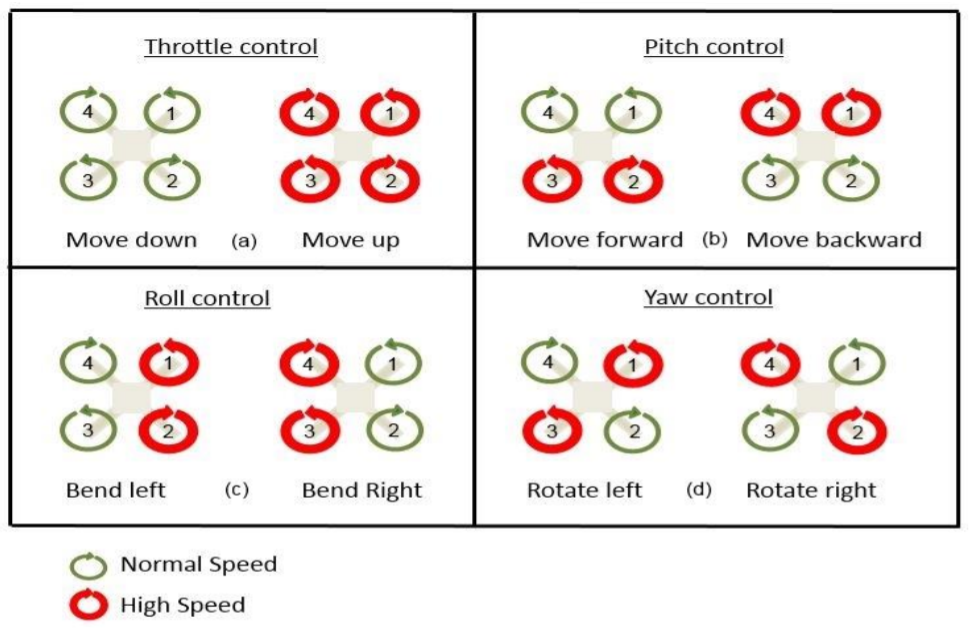
\includegraphics[scale=0.5]{images/motor_signals.PNG}
    \caption{Controlling the UAV \cite{fcDesign2019}}
    \label{fig:motor_signals}
\end{figure}
\newline
In order to be able to model the system and define the control objectives, it is important to get a sense of the parameters that determine
how the UAV moves. For that, we have throttle, pitch, roll, and yaw. These are all illustrated by figure figure \ref{fig:motor_signals} a, b,
c, and d respectively. Throttle dictates the angular velocity of all of the motors. It affects flight velocity as well as the altitude of the
UAV. Pitch is what allows the UAV to move forward or backward. In order to move forward, the flight controller would instruct motors 2 and 3
to accelerate while keeping motors 1 and 4 at a constant angular velocity. The opposite is true for flying backwards. Meanwhile, roll controls
lateral movement. In order to fly to the left, the flight controller would instruct motors 1 and 2 to accelerate while keeping motors 4 and 3
at constant velocity. The opposite is once again true for flying to the right. Perhaps most interesting would be how yaw controls the direction
that the UAV is facing. It was previously discussed that the opposing motor orientations allow the UAV to negate the torque and obtain stable
flight. Yaw takes advantage of this by accelerating either the clockwise rotating motors or the counter-clockwise rotating motors in order to
rotate right or left respectively.
\newline
\newline
With the parameters defined, Zimmerman presents a frame of reference for the UAV \cite{zimmerman2016}. This may be seen in figure \ref{fig:ref_frame}
\begin{figure}[h]
    \centering
    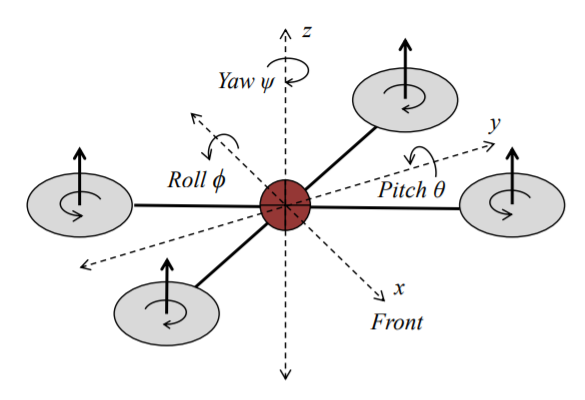
\includegraphics[scale=0.5]{images/quad_ref_frame.PNG}
    \caption{UAV reference frame \cite{zimmerman2016}}
    \label{fig:ref_frame}
\end{figure}
They define pitch to be $\theta$, roll to be $\phi$, yaw to be $\psi$, and throttle to be $T$. These are the current values of the parameters.
They then define $\theta_c$ to be the user commanded pitch, $\phi_c$ to be the user commanded roll, $\psi_c$ to be the user commanded yaw, and
$T_c$ to be the user commanded T. Lastly, they define $ \dot{\theta}, \dot{\phi}, \dot{\psi}$ to be the rotational velocities. According to
Zimmerman, the first set of control goals may be summarized by equation \ref{eq:ctrl_goals_1}.
\begin{align}
    \dot{\theta}&=0                      &  \dot{\phi} &=0                 &  \dot{\psi}&=0\\
    \label{eq:ctrl_goals_1} 
    \theta &\rightarrow \theta_c         & 
     \phi &\rightarrow \phi_c       &  \psi &\rightarrow \psi_c &  T &\rightarrow T_c
\end{align}
In essence, the goal of the flight controller is to drive the parameters to the user specified values. Using these four parameters, the user
is able to maneuver the UAV anywhere in 3D space. In order to achieve the control goals, a PID controller system is implemented. A PID controller is a
control system that updates based on the desired output and the measured output \cite{zimmerman2016}. "PID" stands for proportional, integral,
and derivative. This is because the system has three coefficients (P, I, and D) that characterize how the system reacts to proportional, integral, 
and derivative errors. In their thesis, Zimmerman designed a base PID system with the UAV acting as the plant as seen in figure \ref{fig:basePID}.
\begin{figure}[h]
    \centering
    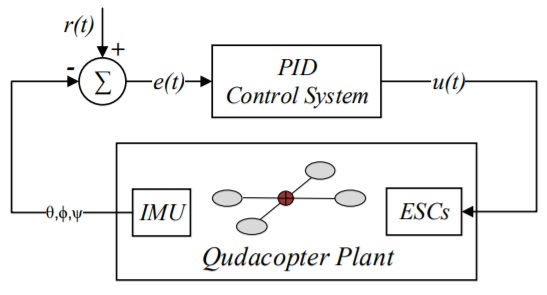
\includegraphics[scale=0.5]{images/basePID.PNG}
    \caption{Diagram of UAV plant and control system \cite{zimmerman2016}}
    \label{fig:basePID}
\end{figure}
Here, r(t) is denoted as the desired setpoint or the user commanded value. e(t) is the error or difference between the output of the UAV plant and
r(t), and u(t) is the input to the plant after the error goes through the PID control system. As we can see, this system also takes into account
the IMU and ESCs for feedback. The ESCs are updated according to u(t) and the corresponding movement is measure by the IMU in order to process it
once again. However, as Zimmerman states, this system is only valid for one parameter. Therefore, there must be one system for each of pitch, roll, 
and yaw. The system is linearized at a current point in time and therefore superposition is upheld. They expand on the control system shown in 
figure \ref{fig:basePID} by incorporating each parameter as well as illustrating how the user commanded throttle $T_c$ fits in the picture. 
\begin{figure}[h]
    \centering
    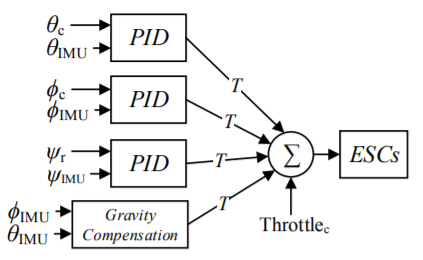
\includegraphics[scale=0.65]{images/controlSysExpanded.PNG}
    \caption{Expanded view of UAV control system \cite{zimmerman2016}}
    \label{fig:expandedPID}
\end{figure}
As we can see from figure \ref{fig:expandedPID}, each PID block takes in the user commanded value of the parameter as well as the parameter's
feedback from the IMU. It then takes in the summation of all of the PID outputs with the user commanded throttle and sends the information to the
ESCs. Zimmerman then goes on to explain how a code for the system may be written for the microcontroller they used for the thesis. While the code
isnt directly compatible with the Raspberry Pi due to differing system architectures, the code will be used as a basis to adapt a version capable
of running on the Raspberry Pi.
\newline
\newline
Now that a control system has been established, there is still the issue of which PID coefficients to use. In order to determine the coefficients,
UAVs often undergo tuning. This is especially important for pilots involved in the sport of drone racing as the UAV's PID coefficients heavily
impact its flight characteristics \cite{Dowling2018}. One method of tuning a UAV is by conducting test flights where the pilot executes sharp
maneuvers, subjecting the UAV's IMU to drastic changes and seeing how the UAV reacts or how quickly it stabilizes \cite{Tuning2017}. Once the tests
are conducted, the pilot would then promptly land and plug the flight controller into a computer to update the PID coefficients in a trial-and-error
manner. One benefit of using a single-board computer rather than a microcontroller for a flight controller is that there would no longer be a need
to plug the flight controller into a separate computer just to update the coefficients. Set up correctly, this could be done mid-flight.


\chapter{Problem Statement and Objectives}
With the rise of research involving multirotor unmanned aerial vehicles comes the development of more advanced flight controllers to aid in the
fabrication of these UAVs. Most (if not all) open source flight controllers are based on microcontrollers while there are no flight controllers
built around single-board computers. Developing a flight controller built around a single-board computer would provide the UAV with access to 
higher level functions such as automated navigation while being lighter and less expensive than microcontroller based flight controllers that
attempt to implement the same higher level functions.
\newline
\newline
This project aims to develop a general purpose flight controller built around the Raspberry Pi and without integrating an auxiliary microcontroller.
To do this, the following objectives must be achieved: 
\begin{enumerate}
    \item The flight controller should be capable of running on a Raspberry Pi 4 without using an auxiliary microcontroller.
    \item The flight controller should be able to sustain stable flight, maintaining a mean error for each parameter (pitch, roll, yaw) of at most 0.001\textdegree
        and a standard deviation of at most 0.4816\textdegree.
    \item The flight controller should be able to respond to commands given by the base station and send back telemetry data.
\end{enumerate}

\chapter{Methodology}

\section{Flight Controller Design}
\begin{figure}[h]
    \centering
    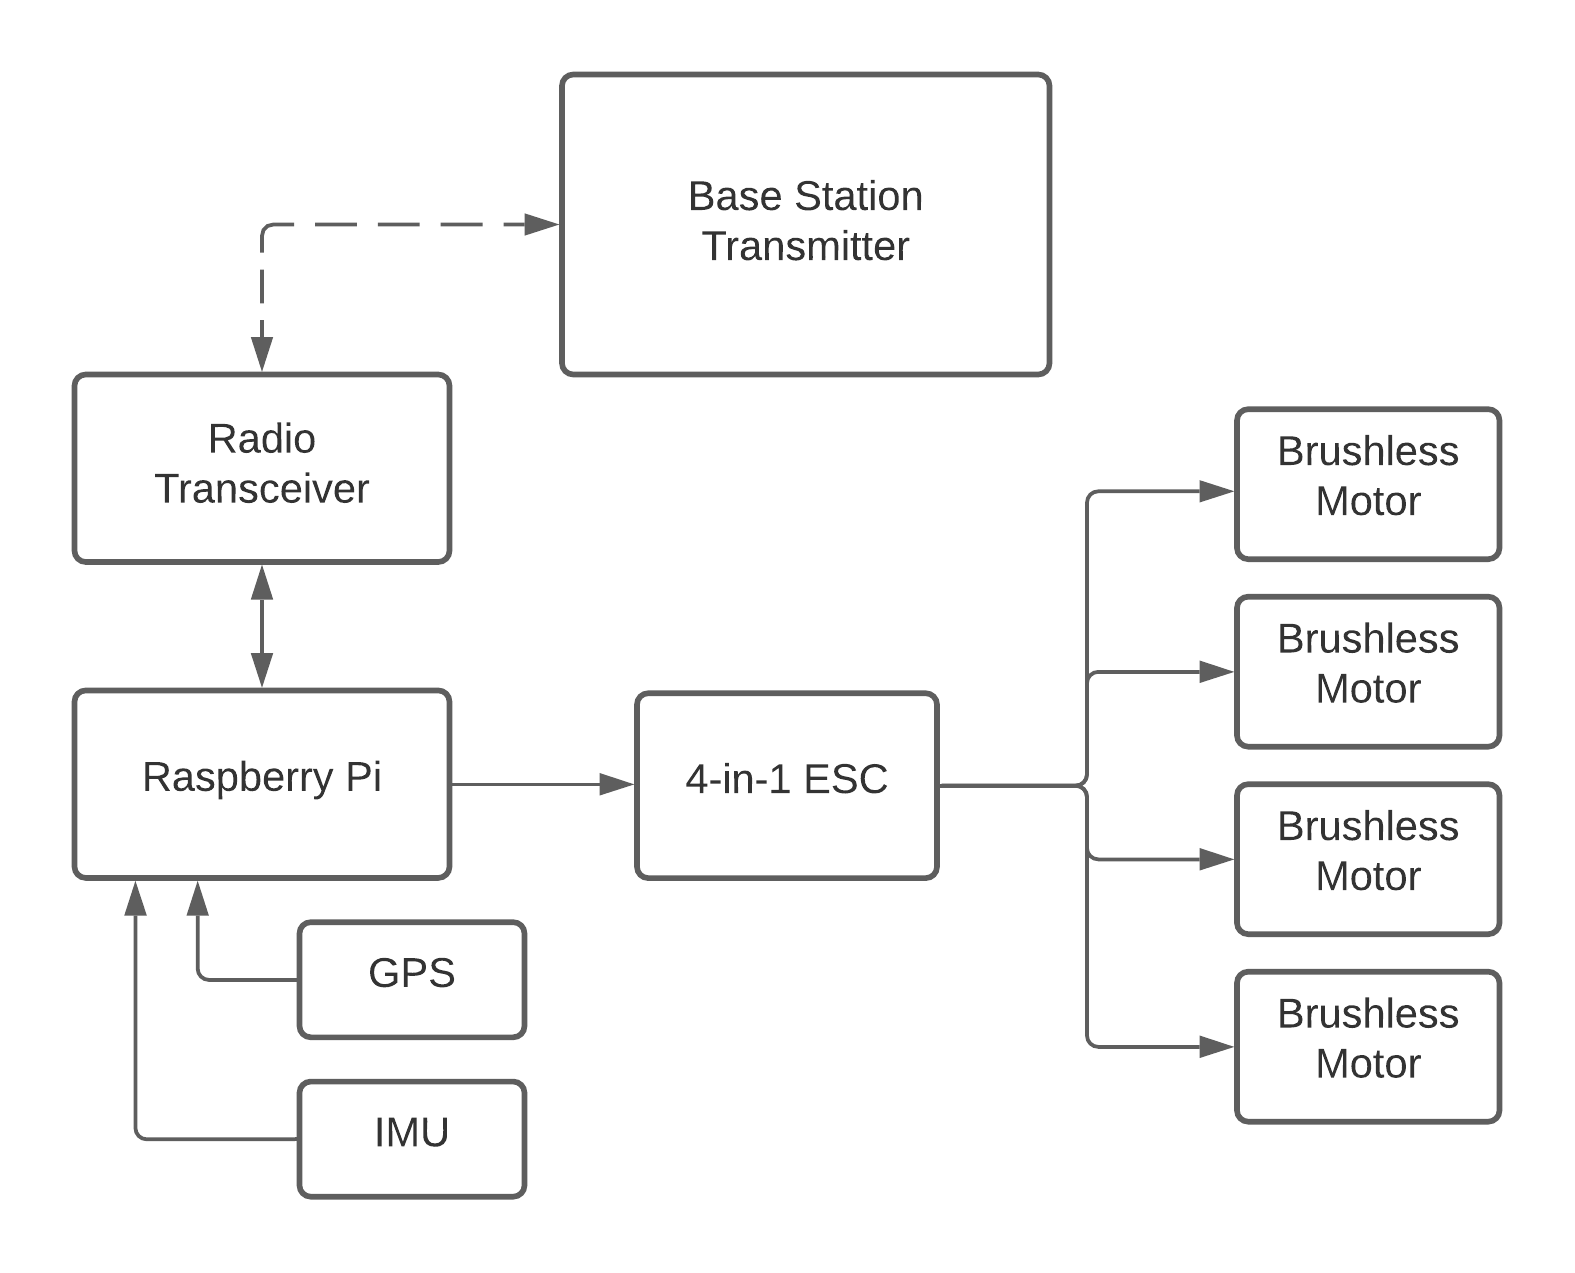
\includegraphics[scale=0.5]{images/FC diagram_finalna.png}
    \caption{Flight controller diagram with ESC module and motors}
    \label{fig:final_FC_diagram_na}
\end{figure}
A circuit board must be designed and fabricated reflecting the diagram seen in figure \ref{fig:final_FC_diagram_na}. As we can see,
the Raspberry Pi draws inertial data directly from the IMU and gathers geographical coordinates from the GPS whenever there is a GPS
signal available. GPS would typically only be available outdoors. The Raspberry Pi will also be directly connected to the ESCs, giving
the Raspberry Pi full authority over them. This is in contrast with microcontroller based flight controllers, where an onboard computer
may only send certain signals. A half duplex radio connection will be established between the flight controller and a base station. 
This will allow the flight controller to take commands from the base station whilst simultaneously sending back telemetry data for 
in-flight debugging. 
\newline
\newline
Once we have established the hardware, the designed control system must then be adapted into code to be run on the Raspberry Pi. 
Integration of the PID control system into the flight control code will be done with aid from Zimmerman's 
derivation and code of his own system \cite{zimmerman2016}. Once the PID control system has been established, the other basic 
functions may then be developed. The ADC will be set up such that it can measure the battery voltage. This will allow the UAV to
send the battery level back to the base station. This function is important as it is vital that the pilot knows how much battery
(and by extension, flight time) the UAV still has. The GPS module will also be set up in such a way that the UAV will be able to
send its current coordinates back to the base station in the event that a GPS signal is detected. This function will be vital for
tracking the UAV in the event of a crash.

\section{Tuning and Experimentation}
\subsection{Communication and UAV Response Test}
During flight, it is important that communication between the UAV and the base station is kept. Thus, there is a need to verify that
packets sent to and from the UAV are consistent with packets sent from and to the base station. This will require a secure shell (SSH) connection with the Raspberry Pi.
On the base station, we will continuously send packets containing the user commanded throttle, roll, pitch, and yaw values. Each
parameter will begin at zero and will be steadily incremented to their maximum value of 1024. Meanwhile, on the flight controller end,
we will continuously receive the data. Once the test is done, we will plot the sent parameter values and the received parameter values
over time to check if there are any discrepancies between the two plots. If a value in the sent parameter values does correspond to a
received parameter value, that packet will be considered lost. The target for this test is that there should be no more than 5\% of
packets lost.
\subsection{Throttle Test}
We must verify that the flight controller is able to command enough throttle from the motors such that the UAV is able to achieve
liftoff. In other words, we must verify that, while under the command of the flight controller, the total thrust generated by all four 
motors exceeds the weight of the entire UAV without a payload. Payload in this instance would be defined as any object on the UAV not
vital for flight. In order to accomplish this, we must first get the weight of the UAV. The UAV will then be fastened upside down to a 
weighing scale. This ensures that thrust from the motors will be directed downwards towards the weighing scale. The throttle will then
be slowly increased while keeping an eye on the weighing scale reading. The generated force must exceed the UAV's weight before the
throttle reaches 100\%.
\subsection{Stability Tests}
\begin{figure}[h]
    \centering
    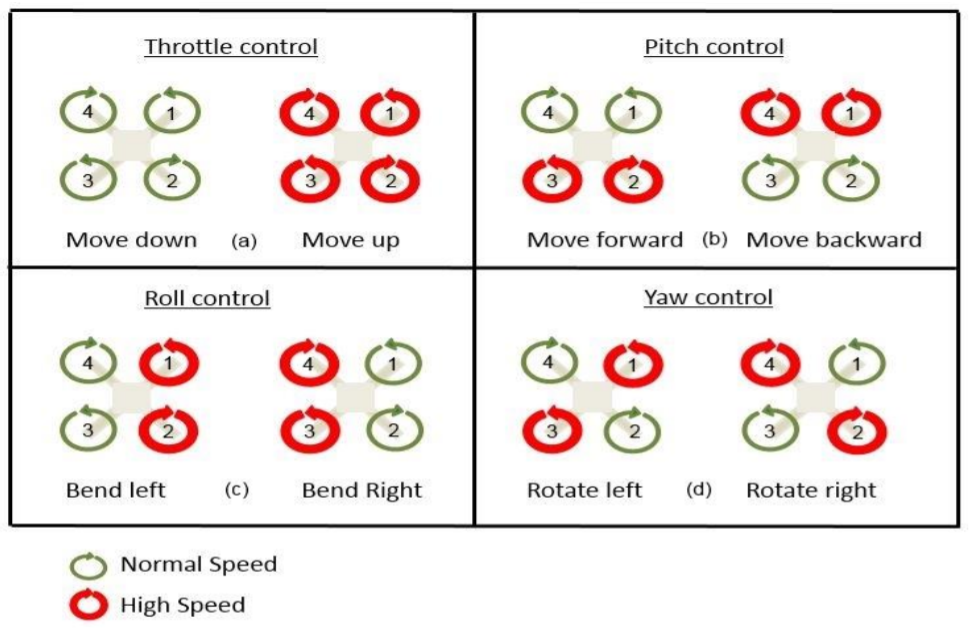
\includegraphics[scale=0.5]{images/motor_signals.PNG}
    \caption{Controlling the UAV \cite{fcDesign2019}}
    \label{fig:motor_signals}
\end{figure}
We may then move on to tuning and stability testing. As mentioned previously, test flights
will be conducted and the PID coefficients will be adjusted to obtain the values that produce the least amount of mean error in the
system. In order to fully test the flight parameters, four tests will be conducted, covering all axes of movement. During these tests, we will be observing the error
responses for the roll, pitch, and yaw PID systems (recall roll, pitch, and yaw from the RRW and from figure \ref{fig:motor_signals}).
Error in the system will be measured by taking the user commanded value of the parameter and subtracting from it the measured steady 
state value for the corresponding parameter from the IMU. An illustration of the experiment is shown by figure \ref{fig:error_diagram}.
\newline
\newline
The first is the \textbf{hover test}. The purpose of this is to establish a baseline for the succeeding tests. In this test, the pilot
will attempt to make the UAV hover in place. While keeping the throttle at a constant value, the pilot will adjust pitch, roll, and yaw
in order to keep the UAV hovering in one spot. Measurement of the exact coordinates is not vital as what we are really looking for is
flight characteristics and whether or not the UAV can achieve stable flight.
\newline
\newline
The next test is the \textbf{pitch test}. The purpose of this test is to isolate pitch from roll and yaw to observe the corresponding
error response. Like the previous test, throttle will be kept at a constant value. In this test, we will also be keeping roll and yaw
at zero. The pilot will then set pitch to a constant value, flying the UAV in a straight line. From this, we may view the steady state error
response of pitch PID system.
\newline
\newline
The third test is the \textbf{roll test}. The purpose of this test is to isolate roll from pitch and yaw to observe the corresponding
error response. For this test, we will be keeping throttle constant and pitch and yaw at zero. Recall that roll is responsible for lateral
movement. The pilot will then set roll to a constant value, flying the UAV left or right. From this, we may view the steady state error 
response of pitch PID system.
\newline
\newline
Lastly, we have the \textbf{yaw test}. The purpose of this test is to isolate yaw from pitch and roll to observe the corresponding
error response. We will be keeping throttle constant and roll and pitch at zero, effectively leaving the UAV hovering in place. Recall that
yaw is responsible for rotational movement. The pilot will then set yaw at a constant value, effectively rotating the UAV either clockwise
or counter-clockwise to see the steady state error response.
\newline
\newline
Data over the course of the tests will then be compiled and the mean error will viewed over time. In this instance, system error 
will be measured in degrees of rotation along a certain axis. Zimmerman's microcontroller based
flight controller has a mean error of 0.001\textdegree with a standard deviation of 0.4816\textdegree. These parameters will be
treated as the baseline. Thus, the mean error of our end system should not exceed 0.001\textdegree and the standard deviation should 
not exceed 0.4816\textdegree. Should the parameter error responses not meet these conditions, the PID coefficients will be changed and the
tests will be repeated. If the conditions are met, the UAV will be considered capable of stable flight.

\begin{figure}[h]
    \centering
    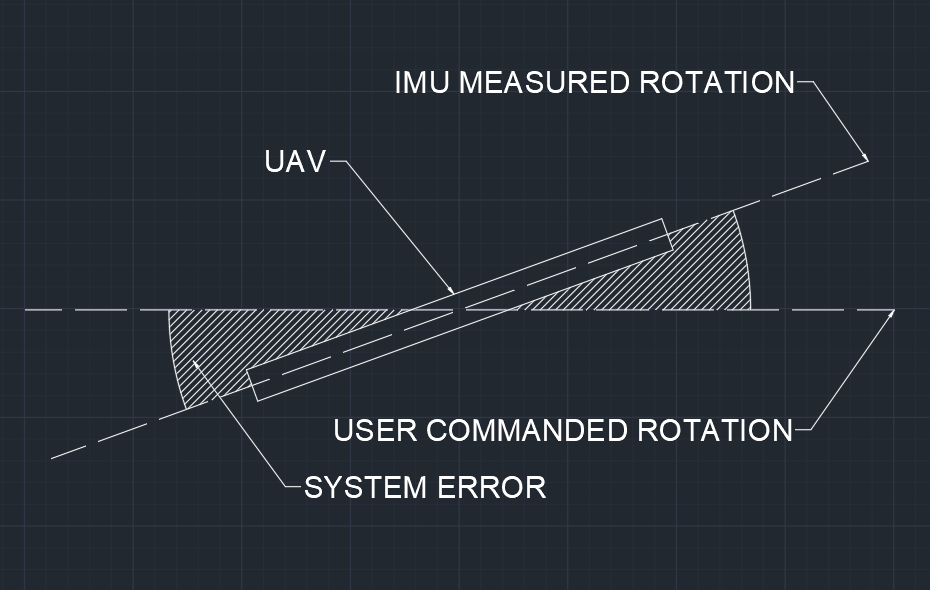
\includegraphics[scale=0.5]{images/error diagram.PNG}
    \caption{2-Dimensional Testing diagram}
    \label{fig:error_diagram}
\end{figure}

\chapter{Preliminary Work}
Previous work has been done to design a flight controller based on the MultiWii flight controller discussed in the RRW. 
The flight controller was designed under the guidance of my advisers as well as the project leaders of Project Diosa.
I designed the flight controller so that it may be used for higher level functions but decided to pivot to focus on more fundamental aspects. 
A diagram of the system may be seen in figure \ref{fig:final_FC_diagram}. It has an integrated
Arduino Pro Mini microcontroller as well as an onboard IMU, GPS, ADC, power module, and radio transceiver. A 4-in-1 ESC board was selected over
individual ESC modules because the board is lighter, smaller, and is less costly. Furthermore, less wiring will need to
be done, leading to easier mass production. The motors are 2400KV brushless motors suitable for 5 inch propellers.
For the inertial measurement unit, the MultiWii was connected to an MPU6050 via an I2C interface. The MPU6050 includes
both an accelerometer and a gyroscope. The arduino receives instructions from a Raspberry Pi 4. There are two
options for communication between the Raspberry Pi and the Arduino; single wire PPM and PWM over multiple wires. Both
methods were tested to find the method with the most stable signal. It was found that the signals gained from PWM over
multiple wires was noisy. PPM gave a much more consistent signal and so it was chosen as the mode of communication.
The Raspberry Pi will also be receiving data from a GY-87 module, which contains an accelerometer, gyroscope, barometer, 
and magnetometer which are all accessible via I2C protocol.  
Aside from this, the Raspberry Pi is also connected to a GPS module which, while inoperable during indoor operations,
will prove to be essential during outdoor missions especially when locating the UAV. For communication, the flight controller 
employs a LoRa RA-02 module, which was chosen for its long range capabilities. The LoRa module will be communicating with a 
similar module connected to the base station. A diagram of the system may be seen in figure \ref{fig:final_FC_diagram}. 
\begin{figure}[h]
    \centering
    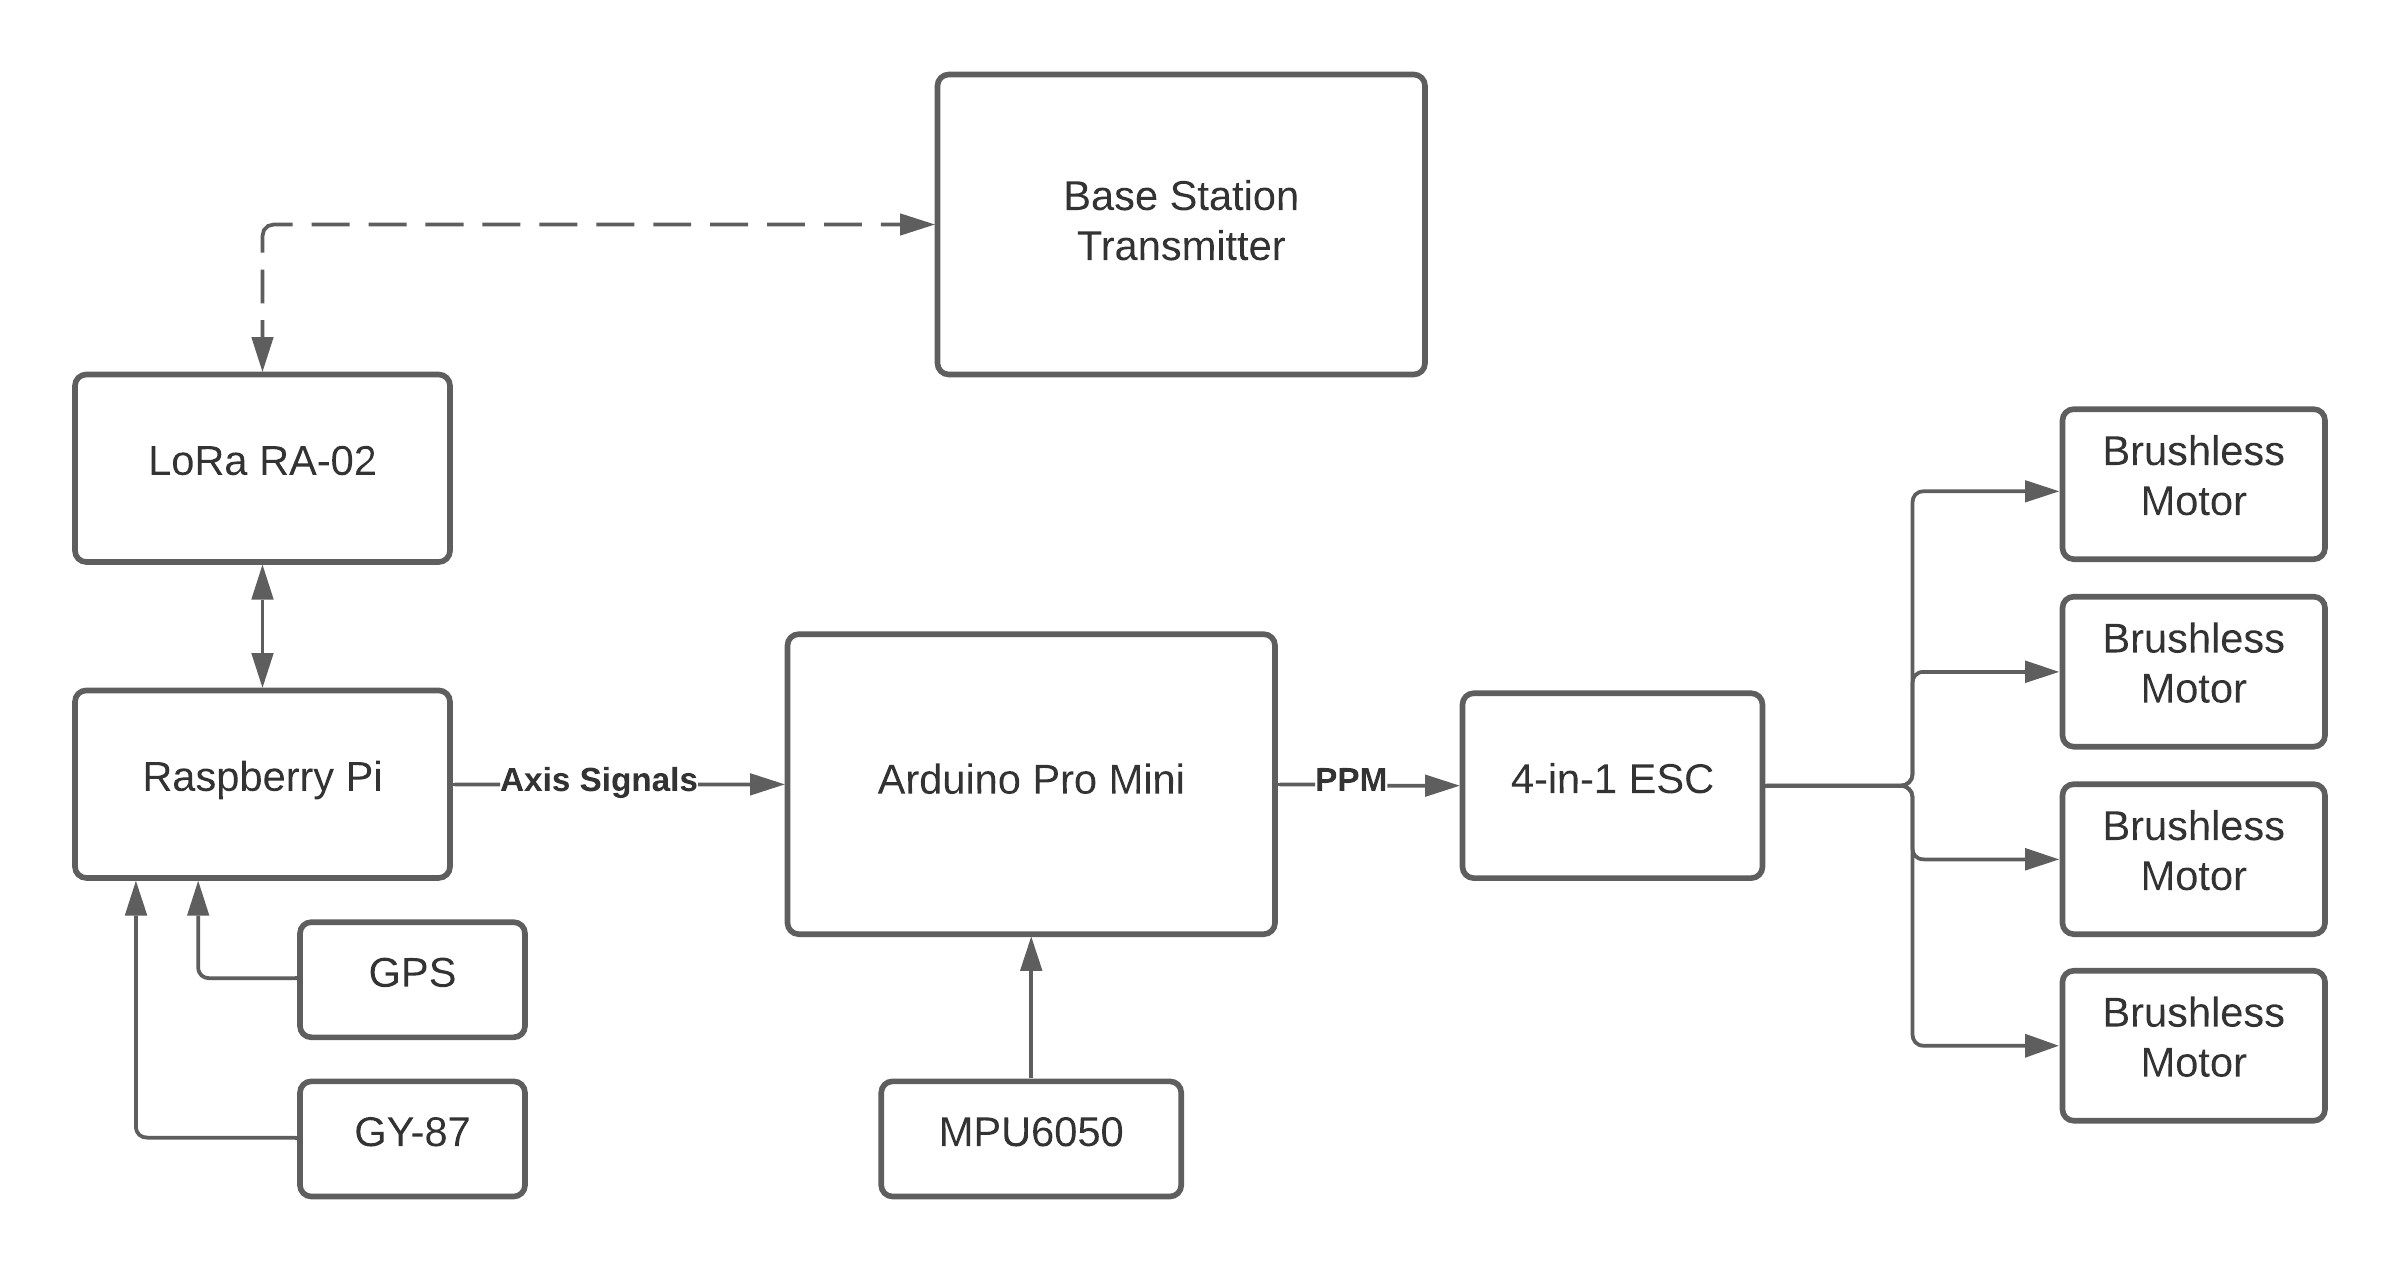
\includegraphics[scale=0.5]{images/final_FC diagram.png}
    \caption{MultiWii based flight controller diagram with ESC module and motors}
    \label{fig:final_FC_diagram}
\end{figure}
\newline
\newline
The Raspberry Pi is running the latest version of Raspbian. It also uses ROS (robot operating system) for
the UAV's processes. ROS is an open source robotics framework that was designed to be modular and flexible, taking into
account the multitude of processes that a robot needs to run. In the case of this project, the modularity allows for
easier integration of different modules and functions. This in turn means that the source code will be easier to maintain
as more and more functions are added.
\newline
\newline
Much of the existing design may be kept. However, the goal of this project is to remove the need for an auxiliary microcontroller.
Thus, the flight controller must be redesigned and refabricated. The Arduino Pro Mini and MPU6050 will be removed and the Arduino's 
functions will be delegated to the Raspberry Pi 4. While the existing system has not undergone quantitative tests, it has been 
confirmed to be able to run the motors at a speed necessary for flight.

\chapter{Timeline}
\section{Gantt Chart}
\begin{figure}[h]
    \centering
    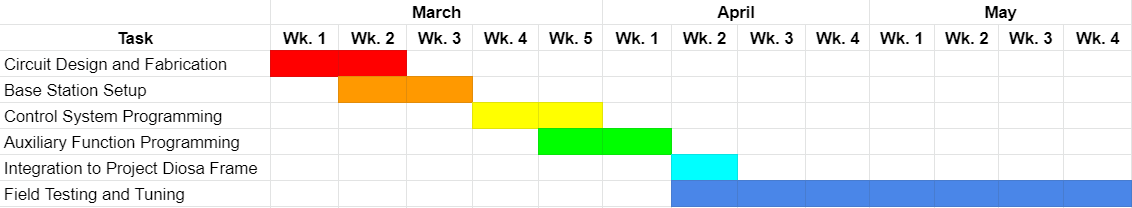
\includegraphics[scale=0.6]{images/gantt_chart.PNG}
    \caption{Project gantt chart}
    \label{fig:gantt_chart}
\end{figure}
\section{Halfway Deliverables}
By the first week of April, the flight controller should be able to achieve the following specifications:
\begin{enumerate}
    \item Flight controller board should be designed and fabricated
    \item UAV should be able to collect inertial data from the integrated IMU
    \item UAV should be able to receive instructions from the base station and send back telemetry data. Packet loss must not exceed 5\%.
    \item UAV should be able to generate thrust greater than its total weight
\end{enumerate}

\section{End of Project Deliverables}
In addition to the deliverables listed above, by the end of the project, the project must have accomplished
the following:
\begin{enumerate}
    \item UAV should be able to collect its geographical coordinates via the GPS module and send the data back to the base station. Received UAV
        coordinates should be within 5m of actual UAV coordinates.
    \item UAV should be able to perform stable flight while correctly receiving pitch, roll, throttle, and yaw instructions (as stipulated In
        chapter 4.2.3)
\end{enumerate}
\printbibliography[
heading=bibintoc,
title={Bibliography}
]

\end{document}

